% !TEXroot=main.tex
\section{Lokalisierung}
{	
	\subsection{Positionierung auf einer Karte}
	{
		
	Um den Roboter Korrekt auf der Karte zu Lokalisieren, wird die Monte-Carlo-Lokalisation verwendet. Als Messpunkte dienen die Daten des LiDAR-Sensors. In der beigefügten Abbildung, wird das vergleichen von Sensordaten und Karte deutlich.
		\begin{figure}[H]
			\centering
			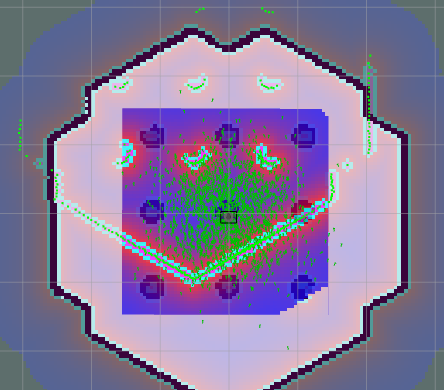
\includegraphics[height=5cm]{Bilder/costmap_monte_carlo_example.png}
			\caption{Costmap mit Sensordaten} 
			\label{pic:coastmontecarlo}
		\end{figure}
		In der Abbildung wird deutlich, dass der Roboter auf der gegebenen Karte (Hintergrund) mittig platziert wird. Gleichzeitig misst der LiDAR-Sensor auch Hindernisse, welche wiederum eine neue Karte der Umgebung bilden. Diese Hindernisse sind hell im Vordergrund zu sehen. Man erkennt, dass diese nicht übereinander liegen und der Roboter deshalb noch nicht korrekt positioniert ist. In Wirklichkeit werden Daten aus der unteren linken Ecke der Karte gemessen. Dadurch werden Positionen in dieser Umgebung sehr wahrscheinlich. Damit der Roboter bei vielen ähnlichen Stellen, was hier nicht der Fall ist, trotzdem korrekt positioniert ist, wird der Roboter zwischen verschiedenen LiDAR-Messungen bewegt. Während der Bewegungen wird errechnet, wo der Roboter sich, ausgehend von den ursprünglichen Vermutungen der Position, befindet. Stimmen auch die neuen Messungen mit der Karte überein, so wird eine Position immer wahrscheinlich, bis der Roboter schlussendlich, sicher positioniert werden kann, da Sensordaten und Karte übereinstimmen. im Falle anderer Roboter können neben LiDAR-Sensoren auch andere Sensordaten verwendet werden.
		
		Die vermuteten Punkte werden dann veröffentlicht, sodass die Navigation darauf zugreifen kann. Diese übermittelten Punkte können in Rviz graphisch dargestellt werden. In der beigefügten Abbildung erkennt man im Hintergrund die erstellte Karte, den Laserscan als grüne Punkte und die geschätzten Positionen (Particlecloud) als grüne Pfeile.
		
	\begin{figure}[H]
		\centering
		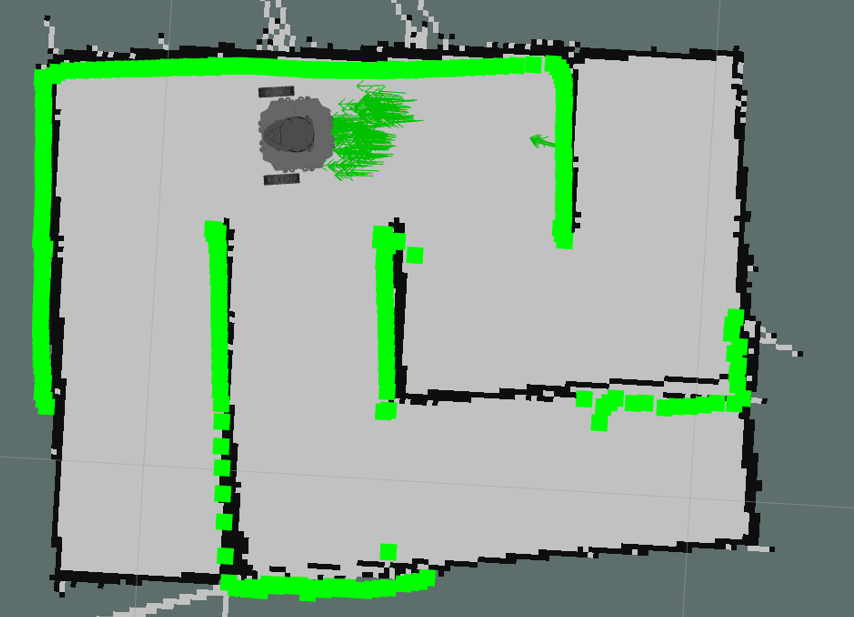
\includegraphics[height=5cm]{Bilder/amcl_clear_pointcloud.png}
		\caption{Particlecloud} 
		\label{pic:amclclearpos}
	\end{figure}

	Es ist zu erkennen, dass gegen Ende der Lokalisierung  die möglichen Positionen eng beieinander sind. Je enger beisammen, desto genauer die Lokalisierung. Die möglichen Positionen werden als Pfeile angezeigt.
	}

	\subsection{Implementierung}
	{
		Die Lokalisierung erfolgt durch das \textit{amcl}-Packet. Dabei handlet es sich um einen Monte-Carlo-Algorithmus. Dieses verwendet die Laserscan-Daten unter der ROS-Topic \textit{/scan}. Diese Topic beschreibt die Laserscan-Daten welche gemessen werden. Ausgegeben wird die \textit{/particlecloud} Topic, welche die möglichen Positionen beschreibt, welche von der Navigation (siehe Abschnitt 7) genutzt werden.
	}
}